%%____________________________________________________________________________||
\section{Systematic uncertainties}
\label{sec:systematics}

We consider two types of uncertainties, all are fully propagated to the likelihood model.
These are normalisation uncertainties and uncertainties associated with the \mht templates for each individual (\njet,~\nb,~\scalht).



\subsection{Systematic uncertainties based on simulations}


We apply several corrections to the simulated samples to correct for known mis-modelling, detector efficiencies and higher order corrections.
These corrections are varied within uncertainties and the resulting variations are propagated through the full analysis, in particular their effect
on the transfer factors as discussed in Sec.~\refe{sec:ewk-method}. The list of simulation based uncertainties is:

\begin{itemize}
  \item{\bf Jet Energy Scale} We vary the jet energy scale \mj and \mmj the μ + jets control regions.  The energies of jets used in the analysis are corrected as a function of their \Pt and $\eta$ following the \textsc{JetMET} POG recommendations. The associated uncertainties are propagated through the analysis.
These uncertainties are typically in the order of the changes are typically about $1-15$\%.

\item{\bf $b$-tagging} Events are reweighted according $b$-tagging efficiencies provided by the $b$-tagging POG.  To test this effect the change in the transfer factors is measured by varying the scale factors within their uncertainties. The relative change is typically about $1-5$\%.

\item{\bf Lepton trigger/identification/isolation efficiency} Systematic uncertainties of 1\% and 5\% are assigned to the efficiency of the muon and electron veto working point efficiency and taken as correlated across all the signal region bin. Data/MC scale factors have negligible scale factors. The procedure is separately applied in the eletron and muon channel. The effect on the $\mj \to \ttbar + $W transfer factors is between $2-5\%$.

\item{\bf $p_\textrm{T}(t)$ reweighting} Variations in the reweighting of $\p_\textrm{T}(t)$ distribution are studied. A conservative systematic uncertainty on this correction is taken as the size of the correction itself.The variation is typically in the range $0-15\%$.

\item{\bf QCD multijet contamination} The \gj control region has a QCD multijet contamination of about 5\%. By applying a large variation of $\pm 100\%$ on the number of QCD multijet events from simulation we derive a conservative systematic uncertainty of 5\%. 

\item{\bf PU reweightings} Events in simulation are reweighted in order to match the distribution of the primary vertex multiplicity observed in data.
By propagating the 5\% systematic uncertainty on the minimum bias cross section used in the PU reweighting procedure we obtain a systematic variation of $1-5\%$.
\end{itemize}


Sec. 12.1 of ~\cite{alphaTnote} shows the exact results of each of these variations for all analysis bins.





\subsection{Systematic uncertainties based on data driven methods}
\label{sec:bkgdnorm-syst}

To derive the normalisation uncertainties for each (\njet,~\nb,~\scalht) bins we use use of ensembles of closure tests. The transfer factors are obtained from simulations and an appropriate systematic uncertainty has to be assigned for each transfer factor to account for limitations in the simulation modelling of event kinematics and instrumental effects. The sensitivity of the transfer factors to systematic sources are determined by performing a set of closure test.
 A large ensemble (\ie hundreds) of closure tests are performed between a number of control (sub-)samples.

Consistency of the set of predictions if then studied and expressed as the ratio $(\nobs - \npre)/\npre$, while considering only
the statistical uncertainties on \npre and \nobs.  If statistically significant biases are observed, further studies are performed to understand and correct for these biases.

The closure tests rely on the \mj, \mmj, and \gj control samples. Specific closure tests probe different sources of uncertainties. 
For example the \mj $\rightarrow$ $\gamma$ + jets tests deal with the consistency
of the prediction of \wej with $\gamma$ + jets. The $\mj \rightarrow \mmj$ tests also addresses the modelling of
vector boson production and the $\mmj \rightarrow \gj$ tests deal with the consistency between the \zee + jets and $\gamma$ + jets samples, which
is a further check on the validity of using the \gj process to predict the \znunu\, + jets process. The muon trigger and reconstruction
efficiencies are also indirectly probed, given that different numbers of muons are required in each of the two sub-samples.
%However, dedicated data-driven methods are used to measure the muon
%trigger and reconstruction efficiencies, with values taken from the
%muon POG.

To test the prediction of \znunu + jets processes with the $W$-enriched \mj control sample
the $\mu^{+}\rightarrow\mu^{-}$ closure test is used. The $0$ b-tag $\rightarrow1$ b-tag and $1$ b-tag $\rightarrow2$ b-tag
tests probe the sensitivity of the transfer factors to the relative admixture of events from the $W$ + jets and \ttbar processes by
varying the number of b-tagged jets within the \mj sample. 

These tests are conservative, as the admixture changes little between the \mj sample and the signal region 
(as there is no extrapolation in \nb), whereas the closure tests use sub-samples with different \nb bins and
therefore different admixtures of $W$ + jets and \ttbar events. \eg, the former uses a $W$-enriched sub-sample (selected by requiring zero
b-jets) to predict yields in a \ttbar-enriched sub-sample (selected by requiring one b-jet).

The $\njet=2\rightarrow\njet=3$ and $\njet=4\rightarrow\njet\geq5$ tests are an aggressive test of the simulation modelling of jet
multiplicities in the \mj, \mmj and \gj samples, which is checked due to the exclusive binning in jet multiplicity. The different \njet
requirements also lead to different admixture of W + jets and \ttbar in the case of the \mj sample.

The TT$\rightarrow$TL closure tests are designed to test the effects of the extrapolation in the
 lepton definition used for the veto in the signal region (see Sec.~\ref{sec:vetoes}) and the selection in the
muon control regions. 

Finally, closure tests that probe the modelling of the \alphat and \bdphi extrapolations in the analysis are also performed. 
In both cases, the test checks if events with genuine \met found in the core of the variable distribution below some 
threshold value can be used to predict the events in the tail (above the same threshold value). 


The systematic uncertainties associated with the transfer factors are determined from ensembles of closure
tests. The statistical precision of these tests is taken into account as it limits the knowledge whether closure is actually achieved or otherwise. 
Ensembles comprising several tests are considered in bins of (\njet,\scalht) to derive a systematic uncertainty for that bin. These systematic uncertainties are then considered a ``normalisation'' uncertainty for the background predictions. These are treated fully fully uncorrelated between the (\njet,~\nb)
categories and \scalht bins. 

%Example of a closure test is given in Fig.~\ref{fig:ZinvclosureDataSymlt400}. The remaining ones can be found in~\cite{alphaTnote}.
All closure tests can be found in ~\cite{alphaTnote}.


In some kinematically restricted bins, such as those with a high jet multiplicity and low value of \scalht, the
limited statistics leads to large systematic errors. These bins are not used in the analysis. 
In the bins populated with a reasonable number of events, the systematic errors determined from the closure tests vary from $10$ to
$40\%$.


\subsection{Systematic uncertainties on the \mht variable}

An additional systematic to be considered is the shape of the \mht distribution in each signal region category. 
A data driven approach is utilized in which the shape of data driven control regions is compared to the \mht shape from simulations.
For each Data/MC ratio of the shape in each signal category bin the first order polynomial is fitted. The result of this fit - a linear bias - 
is then used as systematic uncertainty and propagated through the likelihood model.
This approach has been validated in 8 TeV data. 

Each background in the signal region (\ttbar/W  and \zInv~) is predicted  using several control regions. 
In order to determine the uncertainty in the \mht dimension a combined linear fit is made over all relevant control regions
of the linear function. A requirement of at least 10 events and a non-trivial number of degrees of freedom
 is made to ensure a reasonable fit. Where this requirement is not satisfied the \mht distribution is not used in the signal region.
An \mht requirement of 130 \GeV is made to ensure a similar phase space to the signal region.
The uncertainty on the linear parameter from the fit is then used to define the up and down one sigma variations of the nominal template.
As a conservative estimate, the best fit value of the parameter is added in quadrature to its uncertainty in order to derive the overall variation.

This method has been validated in 8 TeV data and an additional validation is carried out by comparing expected and observed uncertainties
on the linear parameter defining the template variations.




\section{Summary of systematic uncertainties}

Table~\ref{tab:systs} gives an overview of all systematic uncertainties and the correlation model used for the likelihood fit. 

\begin{landscape}
\begin{table}[h!]
  \caption{Summary of the systematics on the transfer factors considered in the analysis,
    with representatives ranges of uncertainties and the correlation assumed,
    for the predictions of the $\ttbar$, W and $\znunu$  background
    components.}
  \label{tab:systs}
  \centering
  \footnotesize
  \begin{tabular}{ ccccccc }
    \hline
    \hline
    Systematic & Method & \multicolumn{4}{c}{Relative uncertainty on transfer factor} & Correlation model \\
     & & $\mj \rightarrow \znunu$  & $\mmj \rightarrow \znunu$ & $\gj \rightarrow \znunu$ & $\mj \rightarrow \ttbar+W$ & \\
    \hline
    \alphat/\bdphi extrapolation & data-driven tests & $5-80\%$ &
    $50-80\%$ & - & $5-80\%$ & un-correlated across \scalht/jet top. \\
    W/Z ratio & data-driven tests & $10-30\%$ & - & - & - & un-correlated across \scalht/jet top. \\
    Z/$\gamma$ ratio & data-driven tests & - & - & $10-30\%$ & - & un-correlated across \scalht/jet top. \\
    W/\ttbar admixture & data-driven tests & - & - & - & $10-100\%$ & un-correlated across \scalht/jet top. \\
    W polarisation & data-driven tests & $5-50\%$ & - & - & $5-50\%$ & un-correlated across \scalht/jet top. \\
    Jet energy scale & MC variations & $<15\%$ & $<10\%$ & $<15\%$ &
    $<15\%$ & fully correlated \\
    B-tagging efficiency & MC variations & $<5\%$ & $<2\%$ & $<2\%$
    & $<5\%$ & fully correlated \\
    Pileup weights & MC variations & $<6\%$ & $<4\%$ & $<3\%$ & $<10\%$ & fully correlated \\
    Top $p_{T}$ weights & MC variations & $<20\%$  & $<4\%$ & - &
    $<5\%$ & fully correlated \\
    Lepton selection & MC variations & - & - & - & $2-5\%$ & fully correlated \\
    \hline
    \hline
  \end{tabular}
\end{table}
\end{landscape}



%\begin{figure}[h!]
%  \centering
%  \subfigure[\label{fig:ttw13} \ttbar/W]{
%    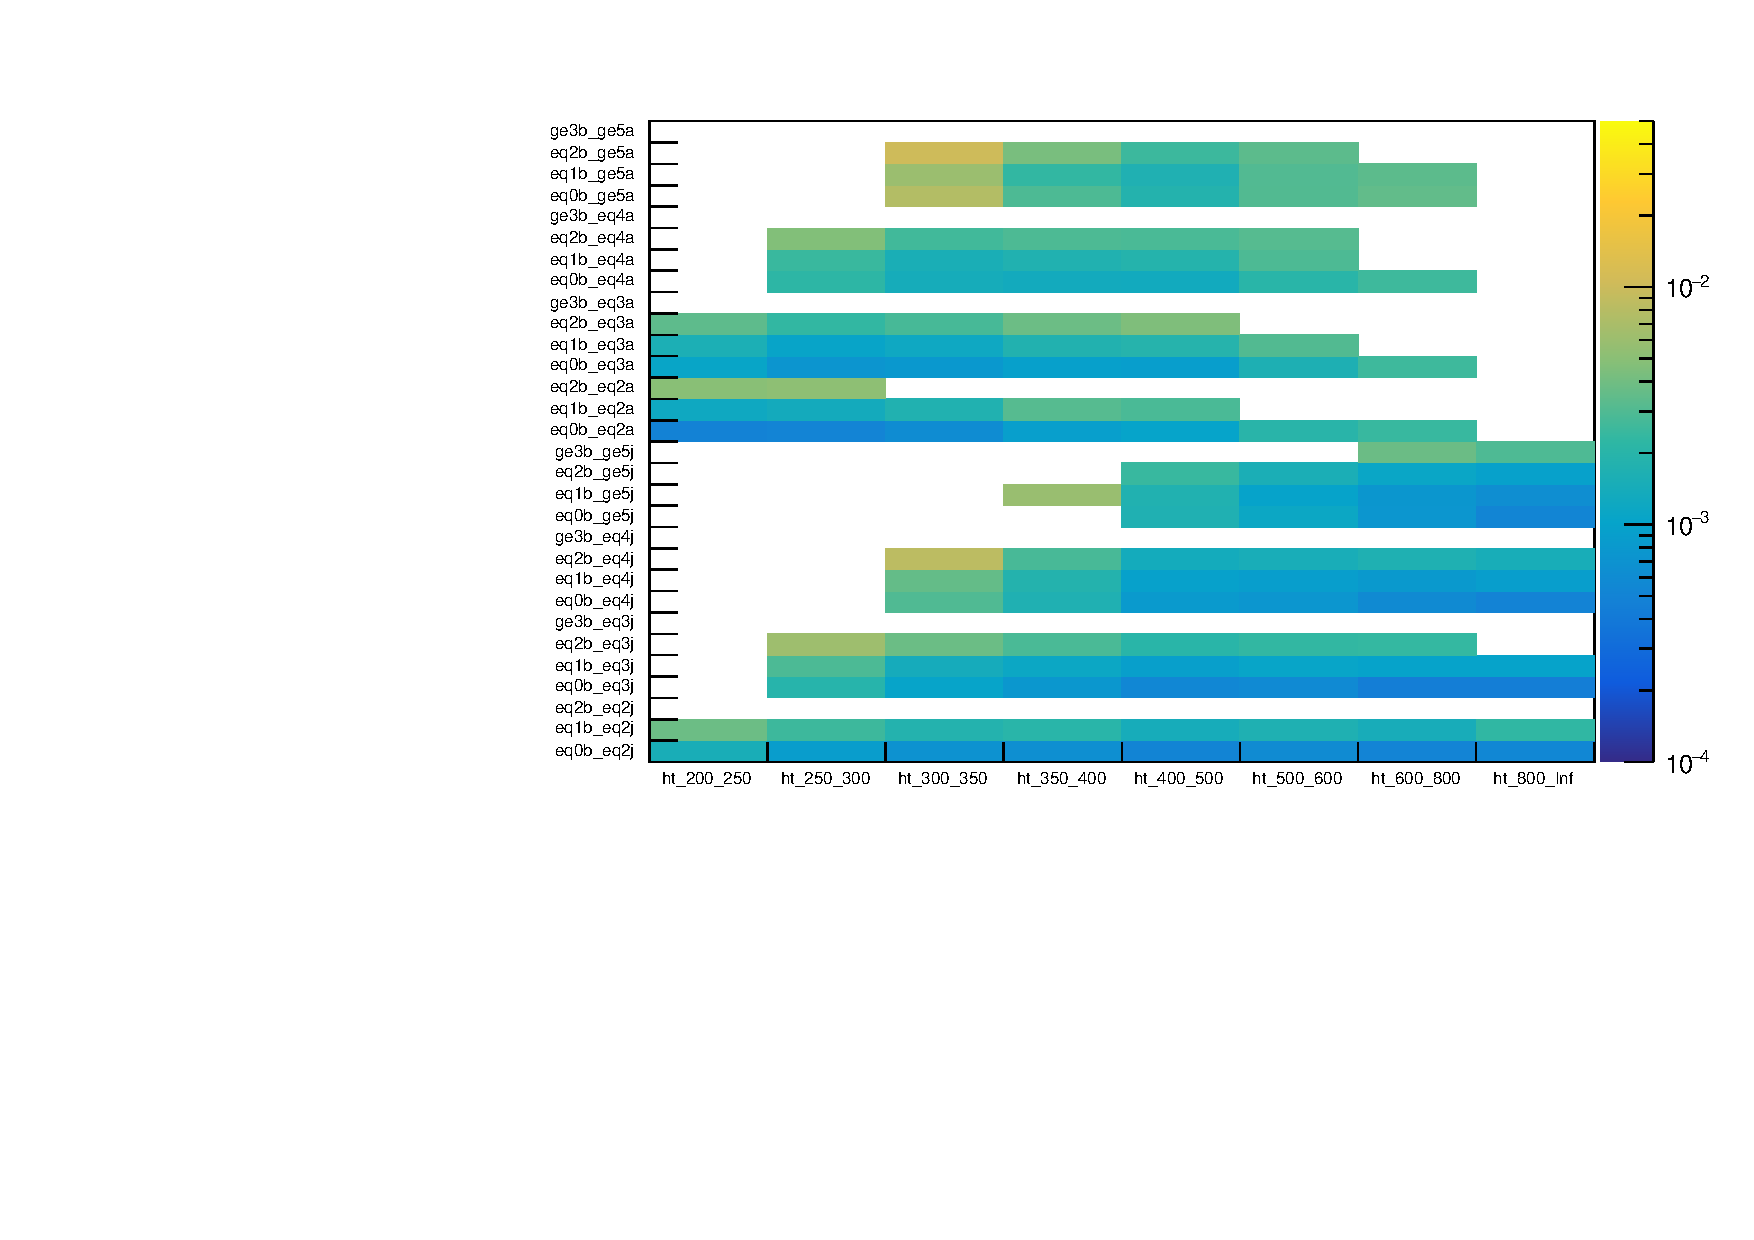
\includegraphics[width=0.5\textwidth]{figures/template13TeV//3fb/frenchFlagErrComplete_Linear2DShiftMean_p1_Ttw.pdf}
%  }~~
%  \subfigure[\label{fig:zinv13} \zInv~]{
%    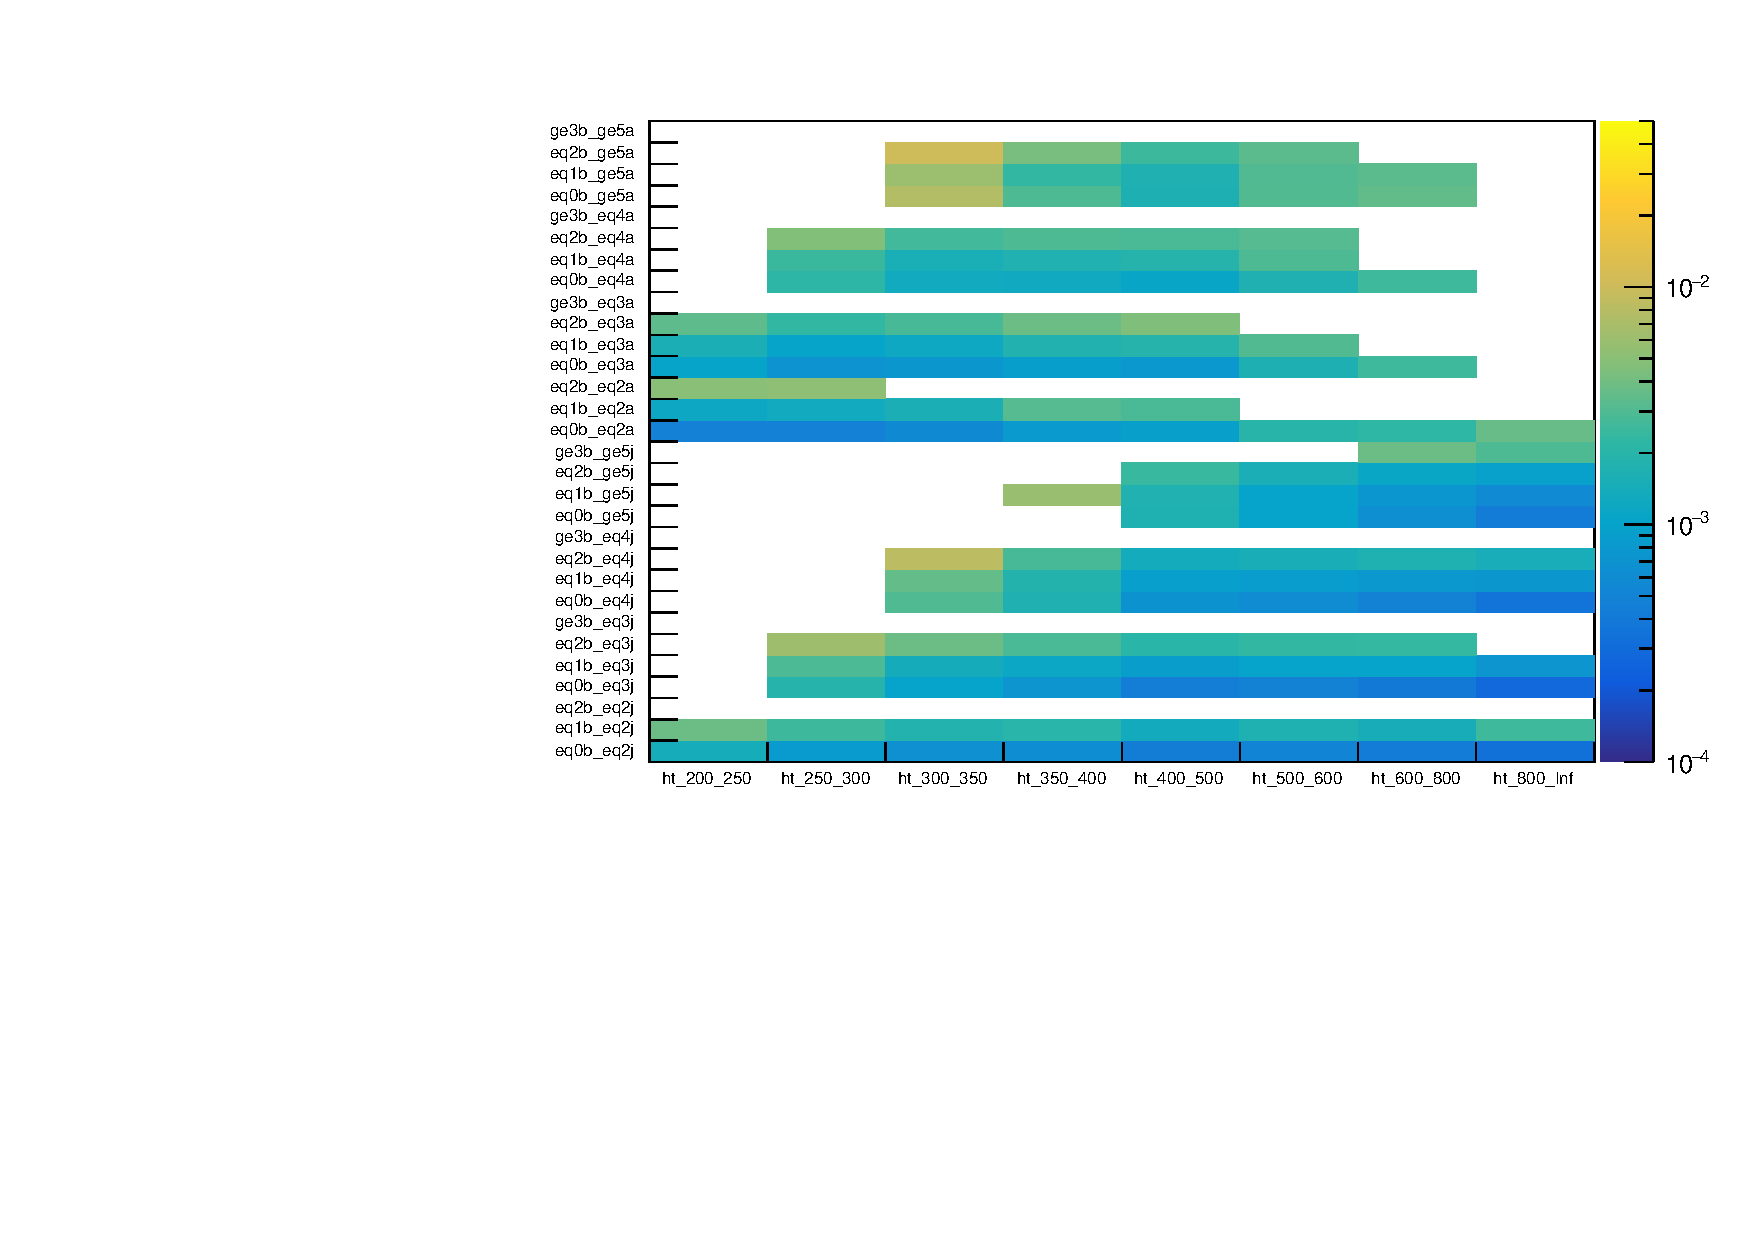
\includegraphics[width=0.5\textwidth]{figures/template13TeV/3fb/frenchFlagErrComplete_Linear2DShiftMean_p1_Zinv.pdf}
%  }\\
%  \caption{\label{fig:expected13} Relative uncertainties per \GeV on the template are shown for \zInv~ in Figure~\ref{fig:zinv13} 
%  and \ttbar/W in Fig.~\ref{fig:ttw13}.}
%  
%\end{figure}%%%

%\begin{figure}[h!]
%  \centering
%  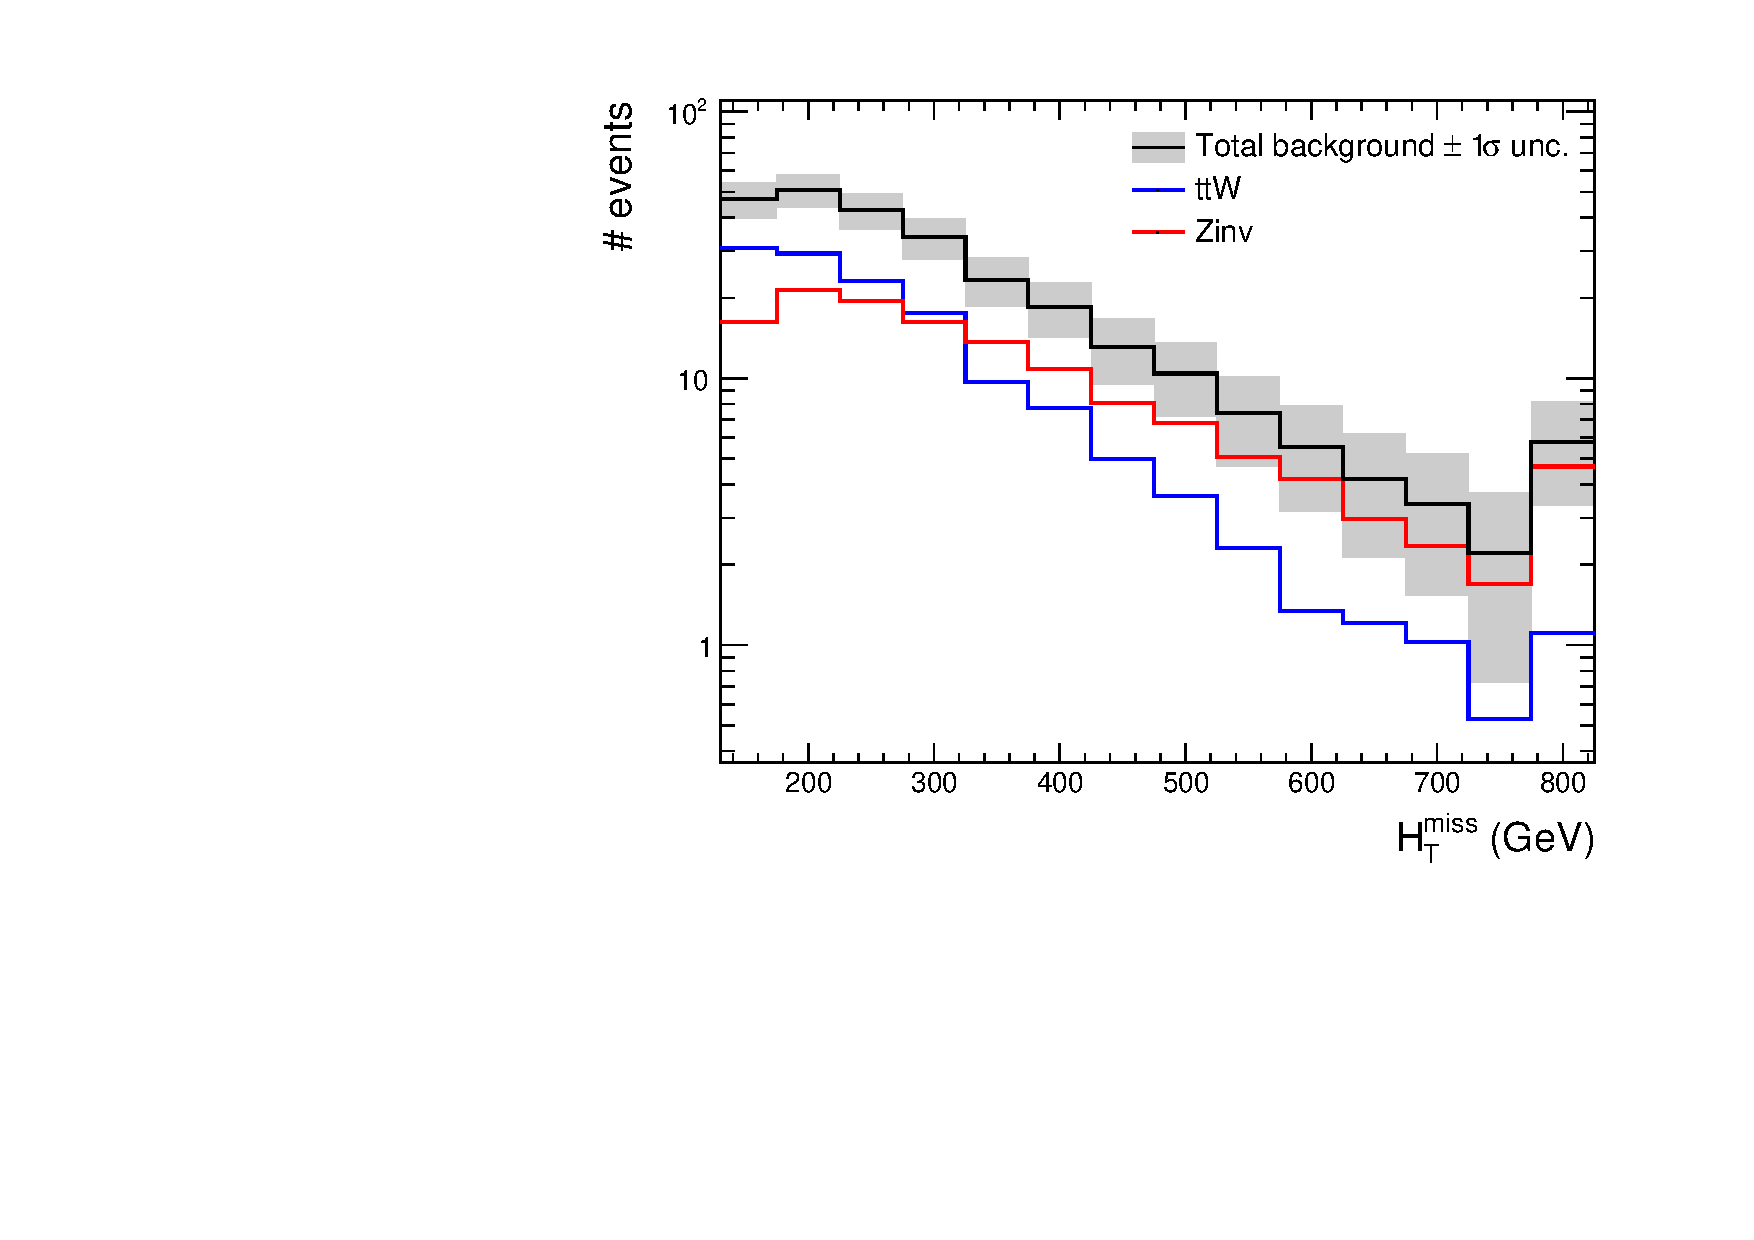
\includegraphics[width=0.5\textwidth]{figures/template/exampleTemplate13TeV.pdf}
%  \\
%  \caption{\label{fig:exampleTemplate13} Example template for 0b,$\ge5$j and $\scalht > 800$\GeV showing the uncertainties from both
%components of the background on the total background prediction.}
  

